\chapter{Evaluation}
\label{cha:evaluation}
This chapter evaluates the prototype implementation of the NanoTorrent protocol.

Section \ref{sec:eval:hypotheses} lists the formed hypotheses that need to be evaluated. Section \ref{sec:eval:method} describes the evaluation methodology. Section \ref{sec:eval:scale} evaluates the scalability of the protocol, and section \ref{sec:eval:hetero} tests the protocol in a heterogeneous deployment. Section \ref{sec:eval:improvements} lists possible improvements that could be made to the protocol, and \ref{sec:eval:discussion} concludes with a discussion.

\section{Hypotheses}
\label{sec:eval:hypotheses}
The goal of NanoTorrent is to deliver files to many \gls{WSN} nodes in a reasonable amount of time, while remaining efficient on battery usage. It should be able to achieve this for many network topologies, which may possibly consist of different types of nodes -- not all of them running a NanoTorrent implementation.

To allow for both fast distribution and heterogeneity in the network, NanoTorrent approaches this problem with a \gls{P2P} file distribution protocol supported by a hybrid peer discovery mechanism. The use of both local peers and remote peers should allow for fast distribution among neighbouring nodes, while still enabling piece exchange with faraway nodes which can help spreading the file in other parts of the network.

\section{Methodology}
\label{sec:eval:method}
To test these hypotheses, the NanoTorrent implementation is run in various experiment configurations inside the COOJA simulator. In each experiment, nodes are tasked to distribute a given torrent and must fully retrieve and verify the contents of the distributed file.

\subsection{AVR Zigduino}
The prototype has been tested and verified in a small network with AVR Zigduino nodes consisting of one border router, one initial seed and three regular peers. The border router is connected to a laptop running the tracker implementation.

Although this set up works, it does not allow a very thorough evaluation of the protocol's capabilities to scale up to larger networks.

\subsection{COOJA simulator}
The evaluations were performed in the COOJA simulator \cite{cooja}. This is a simulation environment for Contiki nodes that emulates the hardware layer of a Contiki platform. It allows Contiki applications to be cross-compiled with the COOJA-specific hardware implementation, and can run these specially compiled versions in various simulated conditions.

COOJA comes with the Contiki distribution and is implemented as a Java application. The simulator interface allows the user to add new motes, place them in a simulated wireless network and configure them. While running a simulation, COOJA shows and records the message logs of all nodes, the timeline of occurred events and the packets transmitted across the network. The recorded information can also be exported for in-depth analysis by other tools.

COOJA simulates the platform and the network at the hardware layer, and interfaces with the compiled C code through the \gls{JNI}. This allows COOJA to run almost any Contiki application, as it behaves just like any other target Contiki platform for cross-compilation. This method of full system simulation is more faithful to real platforms than other simulators such as TOSSIM \cite{tossim} which can only simulate one layer of the platform.

\section{Scalability}
\label{sec:eval:scale}
To be usable in both small-scale experimental setups and large-scale \gls{WSN} deployments, NanoTorrent must be able to scale as more nodes are added to the network.

\subsection{Set up}
Figure \ref{fig:eval:scale:setup} shows the simulation set up. In each experiment, $N^2$ nodes are deployed in an $N \times N$ grid layout such that each node has at most 4 neighbours. Every node has a torrent descriptor for a 2 \gls{KB} file consisting of 8 pieces of 256 \gls{KB}. The top left node acts as the \gls{initial-seed} from which this file will start propagating over the network. This node is also connected with a border router, which connects the \gls{WSN} with the \gls{tracker}. The experiment was carried out for $N =$ 3 to 7, resulting in networks consisting of $9$ to $49$ NanoTorrent peers.

Since all nodes in this set up download the same torrent, file distribution could also be done \emph{without} a centralized tracker. To analyse the benefits or downsides to this approach, every set up is tested once without the tracker and once with both peer discovery mechanisms enabled.

\begin{figure}
    \centering
    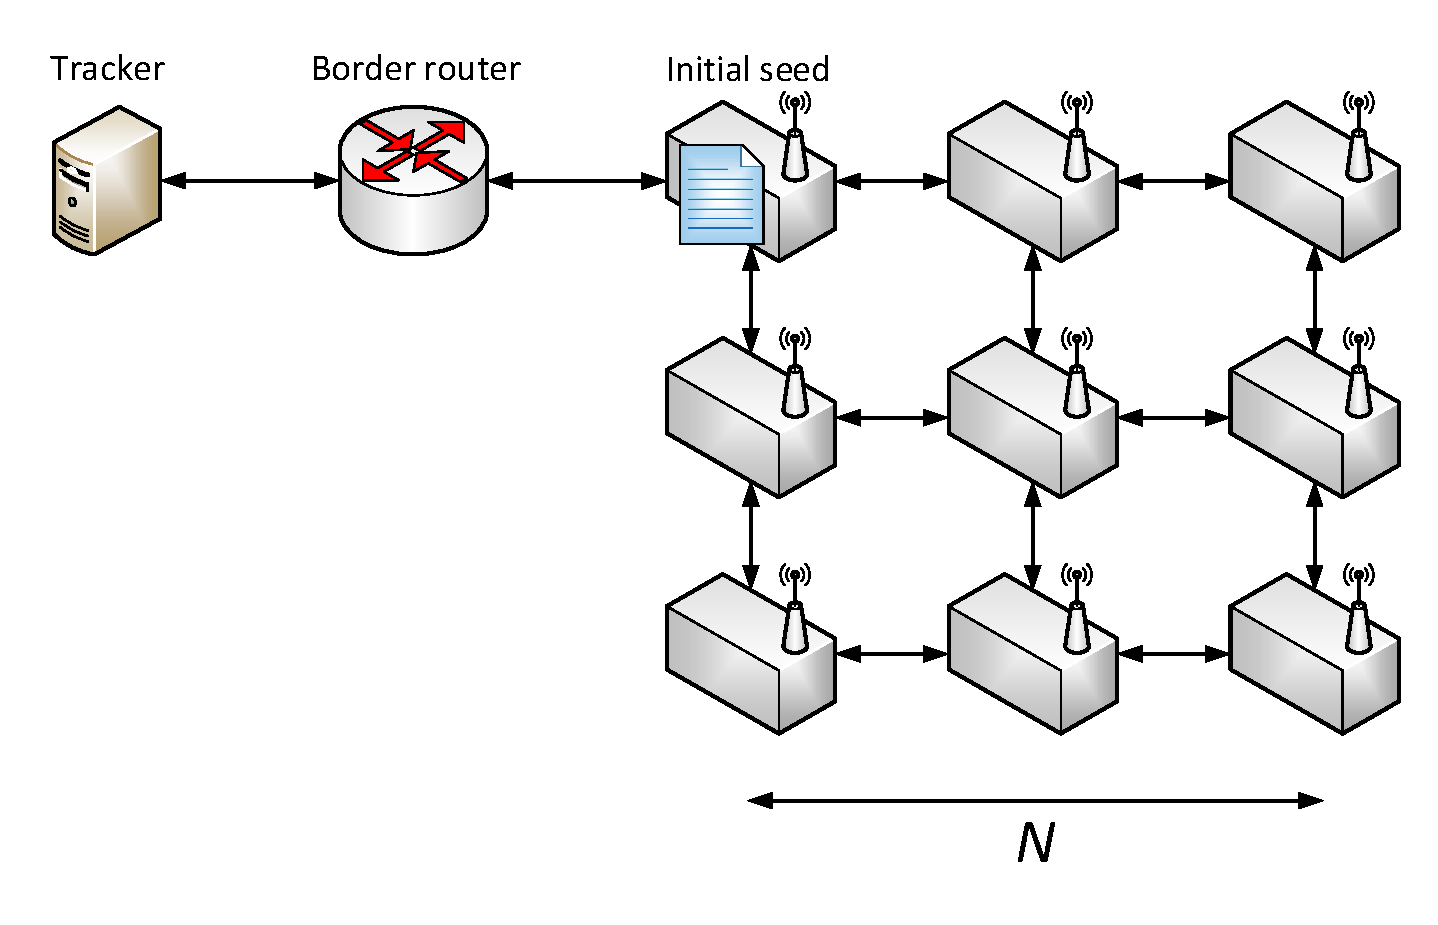
\includegraphics[width=\textwidth]{diagrams/experiment-scale.pdf}
    \caption[Network set up for scalability experiment]{Network set up for scalability experiment. The \gls{WSN} consists of $N \times N$ nodes in a grid layout, with one initial seed.}
    \label{fig:eval:scale:setup}
\end{figure}

\subsection{Results}
Figure \ref{fig:eval:scale:deploy-time} shows the deployment times (i.e. the time to deploy the file to all nodes) for the different network diameters, both with and without the tracker.

Figure \ref{fig:eval:scale:total-transmissions} shows the total number of transmissions sent over the network. This total is broken down into the different upper-layer network protocols in figure \ref{fig:eval:scale:transmissions}. NanoTorrent and NanoTracker indicate messages between peers and with the tracker. \gls{IEEE} 802.15.4 messages consist of link-layer acknowledgements for transmitted frames. \gls{ICMPv6} messages are used to maintain the \gls{IPv6} and \gls{RPL} routing mechanisms. \gls{6LoWPAN} messages consist of fragmented packets which are later re-assembled into larger \gls{IPv6} packets.

Figure \ref{fig:eval:scale:3x3} gives a more in-depth analysis of the download progression in a $3 \times 3$ network. 8 nodes (numbered 3 to 10) receive the file from a single initial seed.

Figure \ref{fig:eval:scale:7x7} displays the completion times of peers in a $7 \times 7$ network. Rather than showing the individual progress of each of the 49 nodes similar to figure \ref{fig:eval:scale:3x3}, this figure only shows the time at which they receive their last missing piece, grouping the results in 5 second intervals. The initial seed is also shown as the only peer completing the torrent after 0 seconds.

\begin{figure}
    \centering
    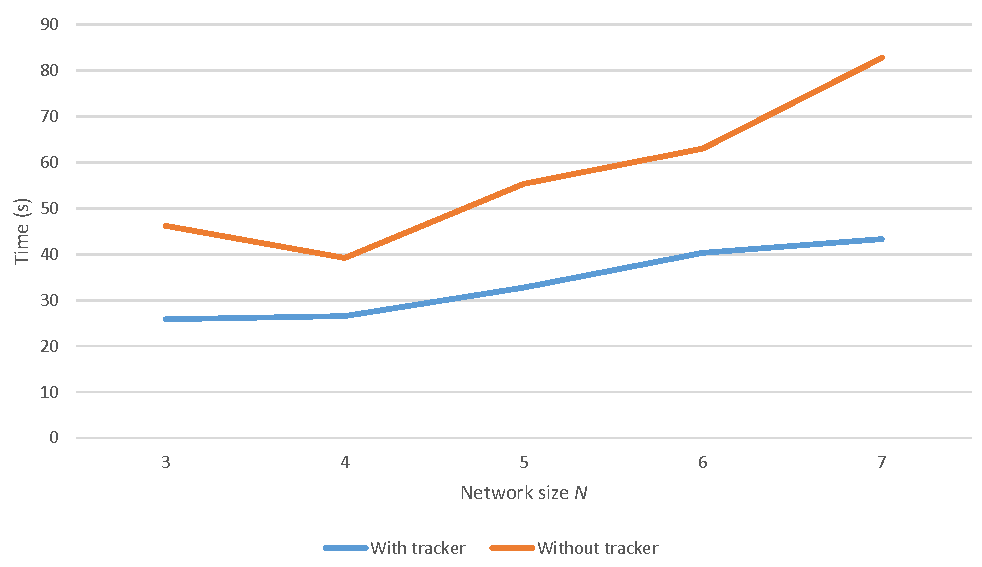
\includegraphics[width=\textwidth]{graphs/scale/deploy-time.pdf}
    \caption[Deployment times for increasing network diameter]{Time to deploy the full file to all nodes for network diameter $N$.}
    \label{fig:eval:scale:deploy-time}
\end{figure}

\begin{figure}
    \centering
    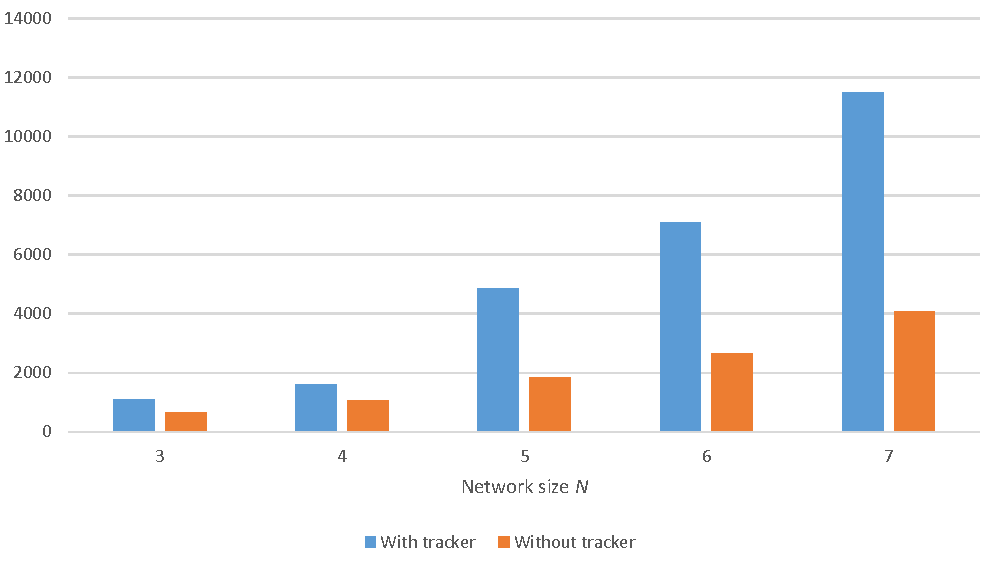
\includegraphics[width=\textwidth]{graphs/scale/total-transmissions.pdf}
    \caption[Total transmissions for increasing network diameter]{Total transmissions sent during deployment for increasing network diameter $N$.}
    \label{fig:eval:scale:total-transmissions}
\end{figure}

\begin{figure}
	\centering
	\begin{subfigure}[b]{\textwidth}
		\centering
		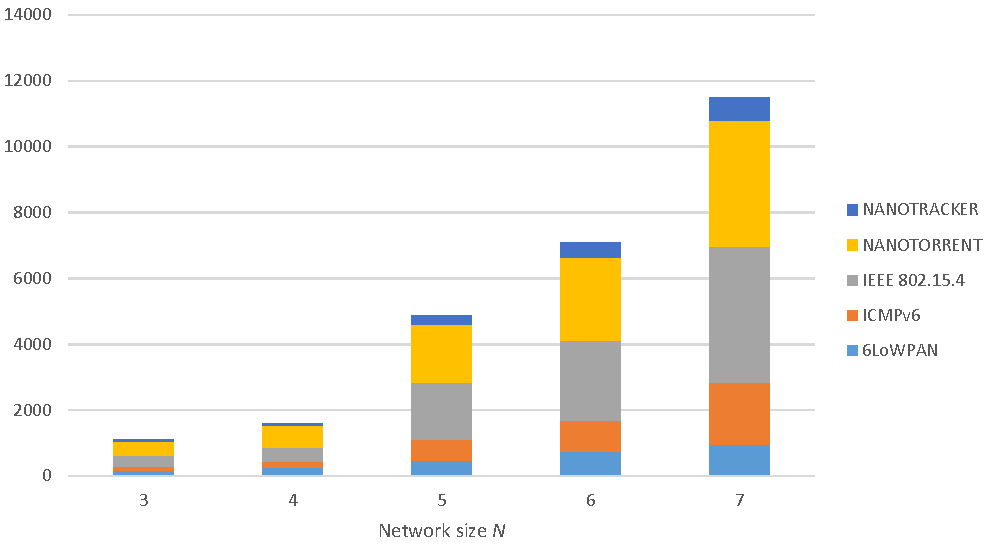
\includegraphics[width=\linewidth]{graphs/scale/transmissions-tracker.pdf}
		\caption{With tracker.}
		\label{fig:eval:scale:transmissions:tracker}
	\end{subfigure}%
	\\
	\begin{subfigure}[b]{\textwidth}
		\centering
		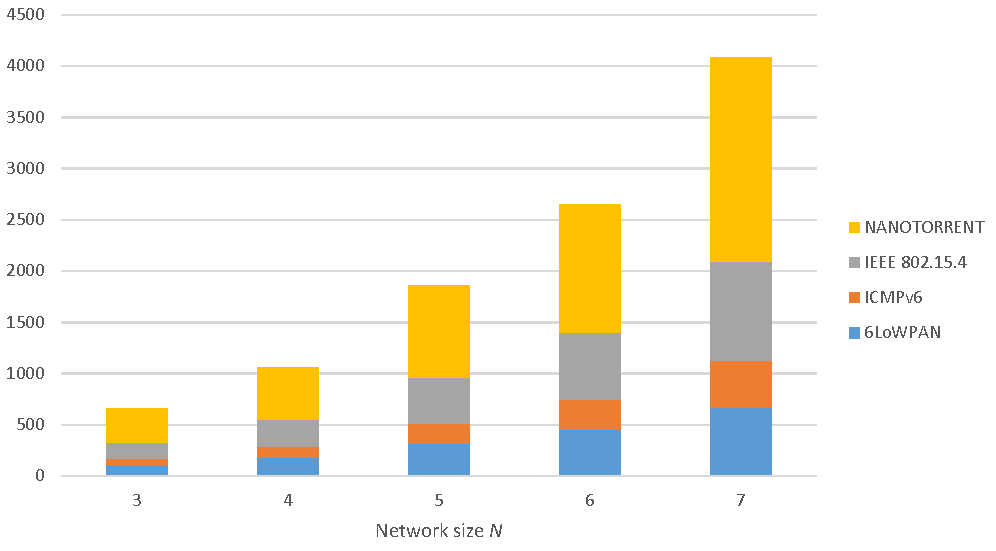
\includegraphics[width=\linewidth]{graphs/scale/transmissions-no-tracker.pdf}
		\caption{Without tracker.}
		\label{fig:eval:scale:transmissions:no-tracker}
	\end{subfigure}
	\caption{Protocol breakdown of transmissions in $N \times N$ network}
	\label{fig:eval:scale:transmissions}
\end{figure}

\begin{figure}
	\centering
	\begin{subfigure}[b]{\textwidth}
		\centering
		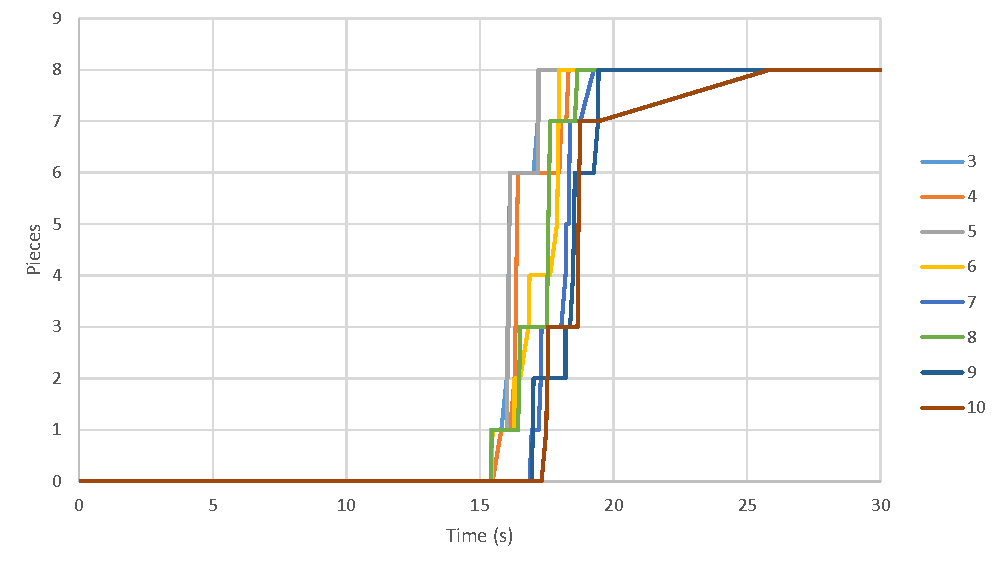
\includegraphics[width=\linewidth]{graphs/scale/tracker-3x3-progress.pdf}
		\caption{With tracker.}
		\label{fig:eval:scale:3x3:tracker}
	\end{subfigure}%
	\\
	\begin{subfigure}[b]{\textwidth}
		\centering
		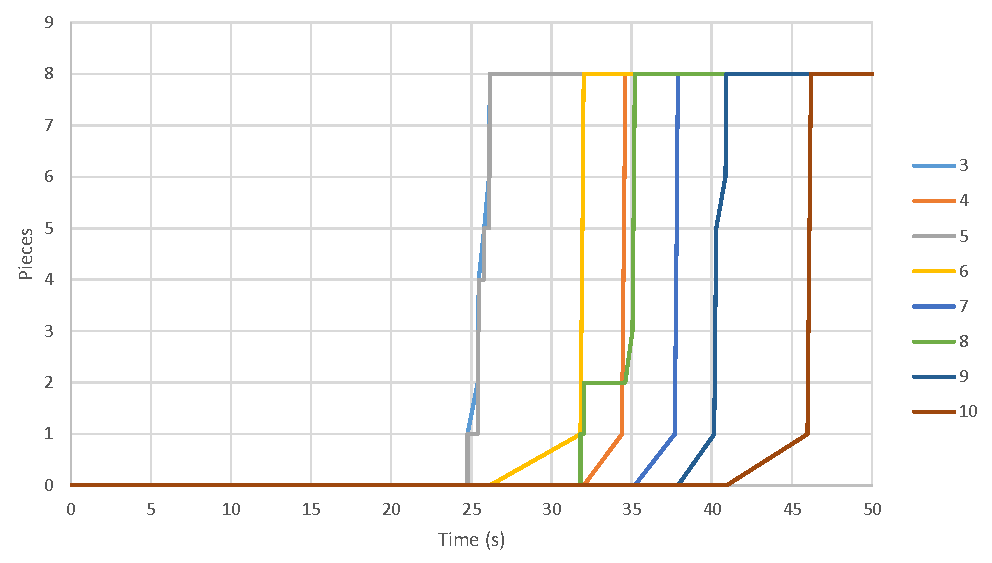
\includegraphics[width=\linewidth]{graphs/scale/no-tracker-3x3-progress.pdf}
		\caption{Without tracker.}
		\label{fig:eval:scale:3x3:no-tracker}
	\end{subfigure}
	\caption[Download progression in $3 \times 3$ network]{Download progression for 8-piece file in $3 \times 3$ network. The different coloured lines indicate the progress of different peers.}
	\label{fig:eval:scale:3x3}
\end{figure}

\begin{figure}
	\centering
	\begin{subfigure}[b]{\textwidth}
		\centering
		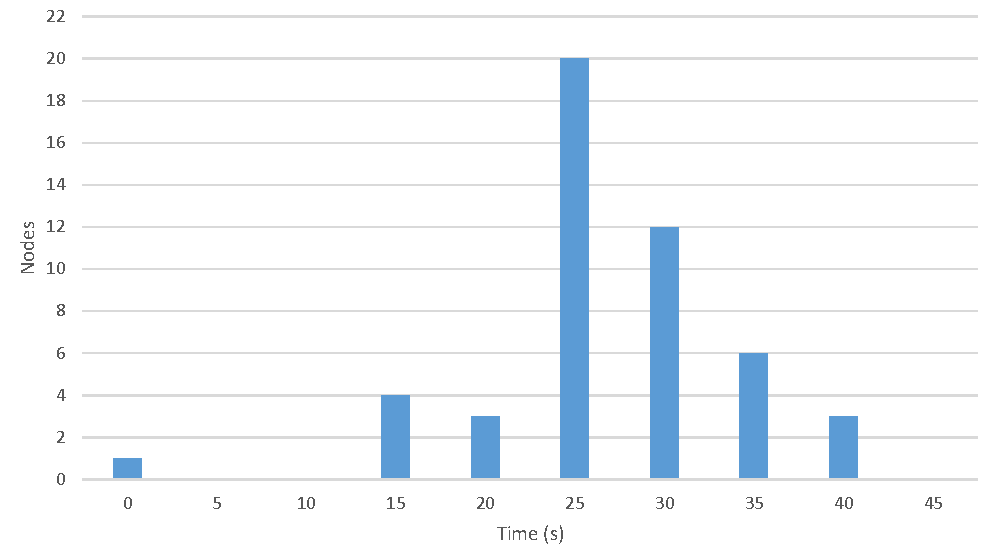
\includegraphics[width=\linewidth]{graphs/scale/tracker-7x7-completion.pdf}
		\caption{With tracker.}
		\label{fig:eval:scale:7x7:tracker}
	\end{subfigure}%
	\\
	\begin{subfigure}[b]{\textwidth}
		\centering
		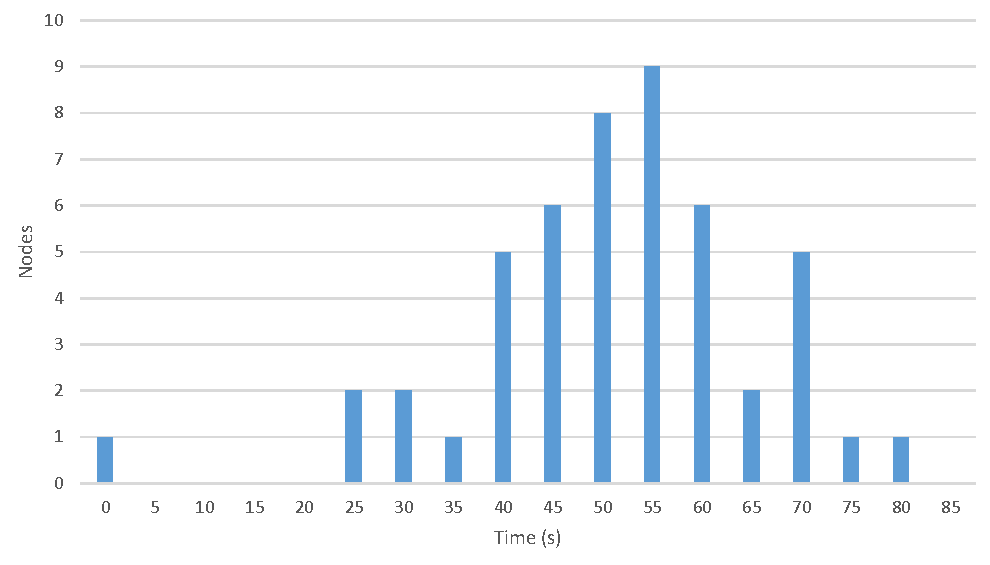
\includegraphics[width=\linewidth]{graphs/scale/no-tracker-7x7-completion.pdf}
		\caption{Without tracker.}
		\label{fig:eval:scale:7x7:no-tracker}
	\end{subfigure}
	\caption[Completion times in $7 \times 7$ network]{Completion times in $7 \times 7$ network. The labels on the X-axis denote the start of an interval, e.g. $0s$ to $5s$.}
	\label{fig:eval:scale:7x7}
\end{figure}

\subsection{Interpretation}
\subsubsection{Deployment time}
Figure \ref{fig:eval:scale:deploy-time} shows that the use of a tracker clearly decreases the total time needed to deploy the file to the whole network. Every peer has additional connections with remote peers from which they can request pieces. Peers on the edge of the network can connect with peers closer to the initial seed, acquire pieces faster and help distribute them to their neighbours.

Without a tracker, every peer must wait until one of its neighbours starts receiving the file. Pieces propagate from the initial seed to the rest of the network as a `wave'. This means that peers on the far edge of the network barely participate in the file distribution, only receiving the file when all other peers have already received it.

Both approaches appear to scale linearly with network size in terms of deployment time. As the network increases in size, the path length between the initial seed and the furthest peer increases linearly as well which is the primary contributor to the deployment time.

\subsubsection{Transmissions}
However, the increased deployment speed from using a tracker comes at a cost in terms of transmitted messages as shown by figure \ref{fig:eval:scale:total-transmissions}. As peers connect with more peers, they need to send more periodic announcements and reply to requests from more peers. While peers on the edge of the network can help balance the load from distributing pieces, communicating with faraway peers is more costly to the network as a whole. The messages between a node and the tracker or its remote peers must traverse the network, taking multiple hops along intermediate nodes which need to use their transmission power to route the \gls{IPv6} packets. These long distance messages account for a lot of overhead transmissions when compared to the tracker-less approach, and this overhead increases with network diameter.

When breaking down these transmissions by protocol, most messages show up as either NanoTorrent or link-layer acknowledgements. The link-layer acknowledgements are an integral part of the network stack, and their usage increases as messages take more hops to get to their destination. This increase is more prevalent in the experiments with a tracker, as NanoTorrent messages need to routed by more nodes to reach a remote peer.

While the number of transmissions without a tracker scales fairly linearly with increasing network size, the number of transmissions when using a tracker seems to increase more than linearly. The additional connections opened by peers cause extra messages on the network which need to be routed across multiple hops.

\subsubsection{Progression}
In the $3 \times 3$ network of figure \ref{fig:eval:scale:3x3:tracker}, all nodes quickly start receiving the file as soon as they receive the first periodic \texttt{have} announcement from the initial seed. Thanks to the tracker, multiple nodes are connected to this initial seed, which means more peers benefit from this initial announcement. In figure \ref{fig:eval:scale:3x3:no-tracker}, the absence of a tracker results in only the two direct neighbours of the seed (nodes 3 and 5) receiving this first announcement. The initial seed communicates only with these two neighbours, which in quick succession request all pieces of the file. However, they take a couple of seconds before notifying their own neighbours, and have already completely downloaded the file before their next \texttt{have} announcement is due. This leaves some room for improvement for fine-tuning the timings of these announcements, to let neighbours more quickly know when new pieces are available.

Figure \ref{fig:eval:scale:7x7} shows the distribution of the completion times of all nodes in a $7 \times 7$ network. For this scenario, the use of a tracker results in a nearly two-fold speed up, distributing the last piece after just 43 seconds as opposed to 82 seconds in the tracker-less experiment. Most peers complete the download around the halfway point, when the `wave front' of the file distribution is the widest at the main diagonal of the grid. In theory, this is when the $N-1$ nodes on the sub diagonal of the square grid are sending pieces to $N$ nodes on the main diagonal, reaching the maximum number of concurrent transfers. When a tracker is employed, the distribution is more skewed as peers use remote connections to exchange pieces.

\section{Heterogeneity}
\label{sec:eval:hetero}
Whereas other distribution protocols for \glspl{WSN} such as Deluge (see \ref{sec:related:deluge}) require all nodes to run the same distribution protocol, NanoTorrent can operate in a \emph{heterogeneous} network consisting of nodes with different tasks and different programs. As long as all nodes properly route \gls{IPv6} traffic across the \gls{WSN}, NanoTorrent peers can communicate with each other even if they are separated by non-NanoTorrent nodes.

\subsection{Set up}
To validate this mode of operation, an experiment was carried out with two clusters each consisting of $5 \times 5$ NanoTorrent peers, which are only connected by a single border router node. This border router routes \gls{IPv6} traffic between the two clusters and to the tracker on the external network. Peers in different clusters can only reach each other through this border router. The set up is shown in figure \ref{fig:eval:hetero:setup}.

\begin{figure}
    \centering
    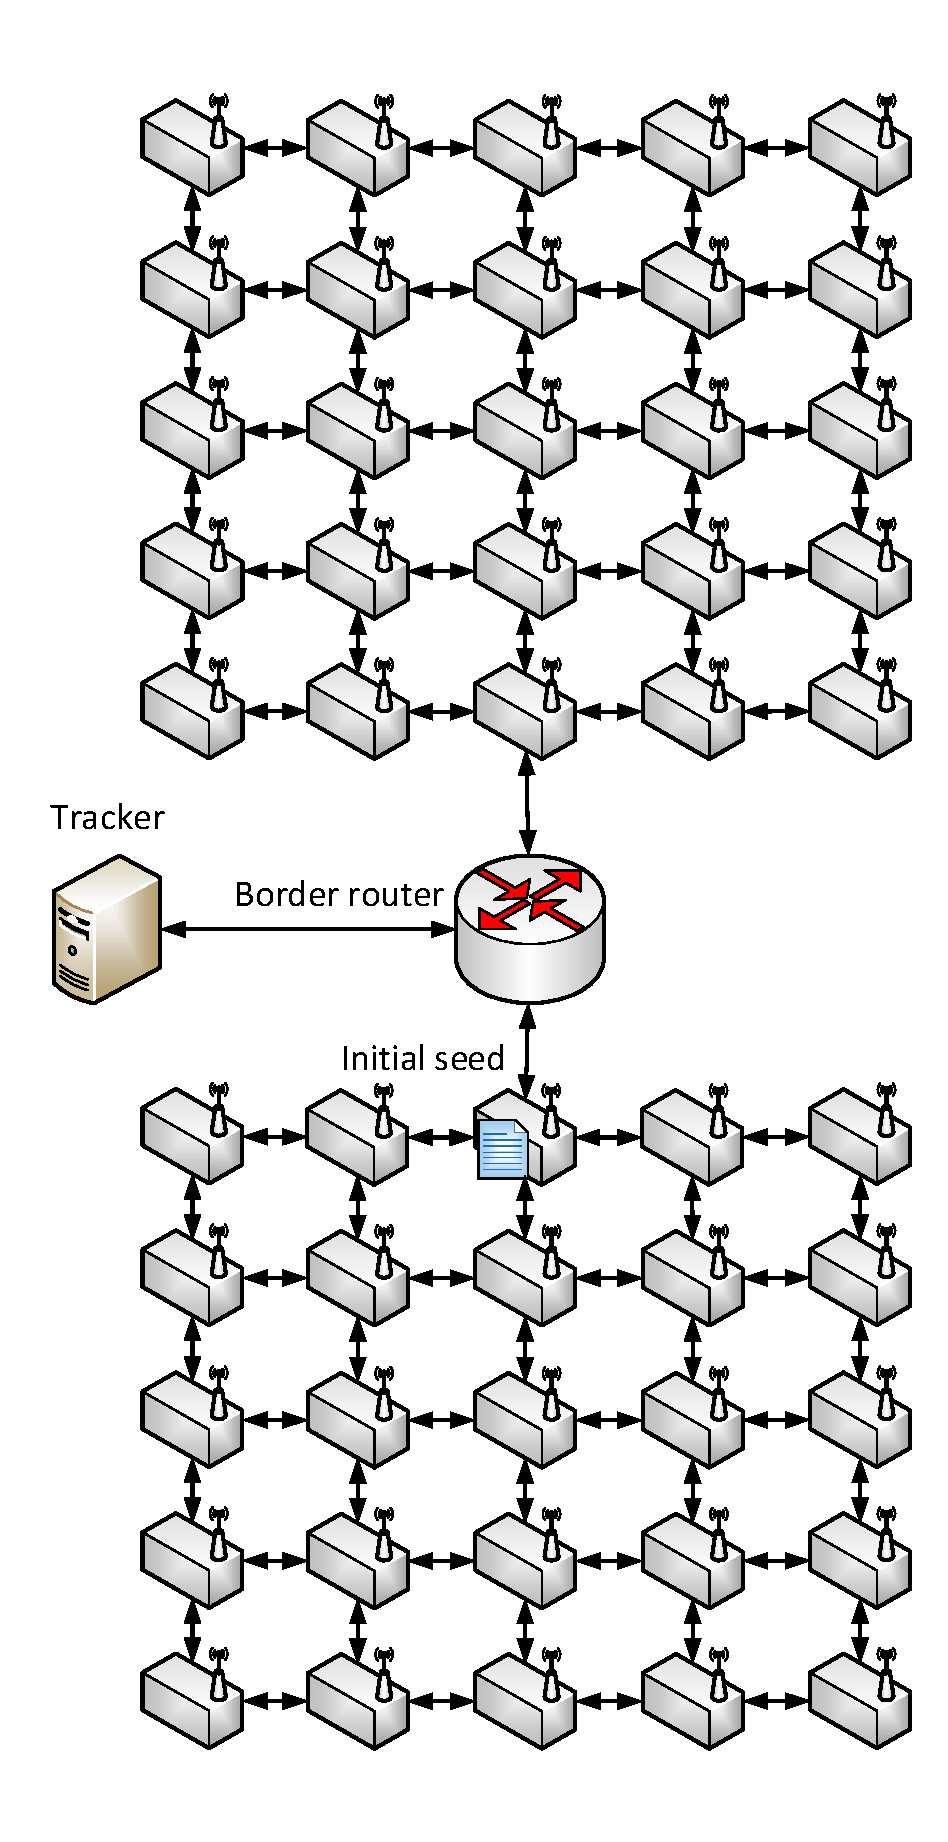
\includegraphics[height=.9\textheight]{diagrams/experiment-cluster.pdf}
    \caption[Network set up for Heterogeneity experiment]{Network set up for Heterogeneity experiment. The \gls{WSN} consists of 2 separate clusters of $5 \times 5$ nodes in a grid layout, with one initial seed in one of the clusters.}
    \label{fig:eval:hetero:setup}
\end{figure}

\subsection{Results}
Figure \ref{fig:eval:hetero:progress} show the download progress of 5 nodes from each cluster of NanoTorrent nodes. Nodes numbered 2 to 26 are in the cluster with the initial seed, while nodes 27 to 51 are in the other cluster.

Figure \ref{fig:eval:hetero:completion} displays the completion times of all the peers in the network, i.e. the time at which a peer receives their last missing piece, grouping the results in 5 second intervals. The initial seed is shown as the only peer completing the torrent after 0 seconds.

\begin{figure}
	\centering
	\begin{subfigure}[b]{\textwidth}
		\centering
		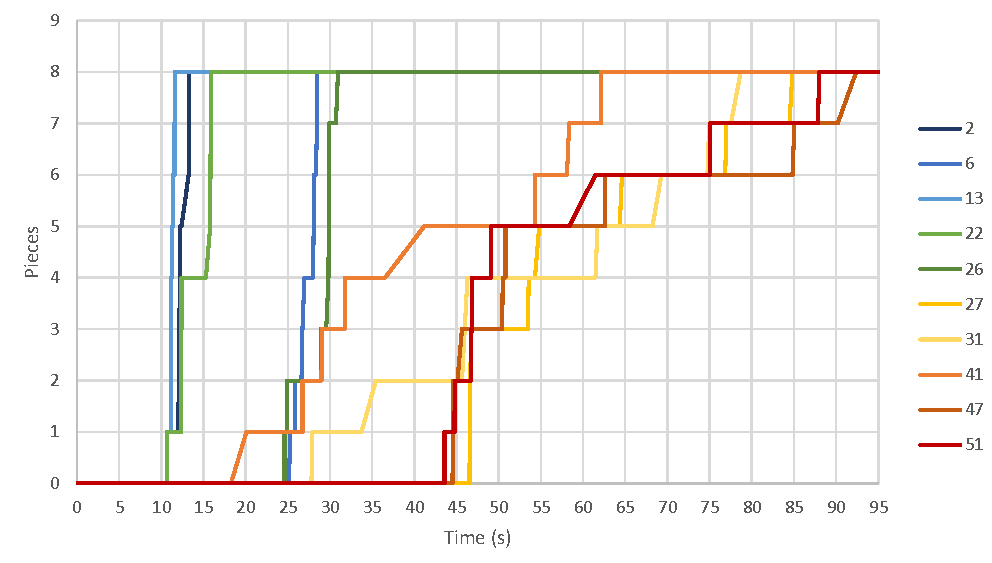
\includegraphics[width=\linewidth]{graphs/cluster/two-cluster-seed-12-progress.pdf}
		\caption{Download progression of a selected number of nodes.}
		\label{fig:eval:hetero:progress}
	\end{subfigure}%
	\\
	\begin{subfigure}[b]{\textwidth}
		\centering
		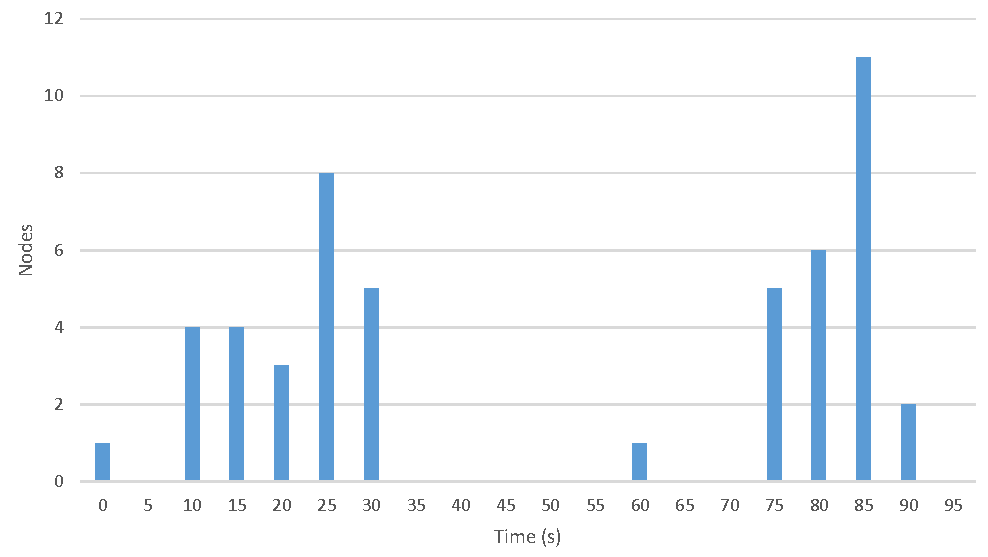
\includegraphics[width=\linewidth]{graphs/cluster/two-cluster-seed-12-completion.pdf}
		\caption{Completion times.}
		\label{fig:eval:hetero:completion}
	\end{subfigure}
	\caption[Results for network consisting of two separate clusters]{Results for a network consisting of two $5 \times 5$ clusters.}
	\label{fig:eval:hetero:results}
\end{figure}

\subsection{Interpretation}
As expected from the results in section \ref{sec:eval:scale}, figure \ref{fig:eval:hetero:progress} shows that peers in the cluster with the initial seed start exchanging pieces quickly. After 35 seconds, the whole cluster has received all pieces of the file and start seeding the torrent.

In the meantime, some nodes in the other cluster manage to connect a peer in the seeding cluster through the tracker and slowly start receiving pieces. Their initial progress is slowed down by the need to pass through the single border router, but quickly start spreading the received pieces to other peers in their cluster. It takes a minute for the first node in this cluster to complete its download, and 30 seconds later the last node receives its last piece.

This slow progression in the second cluster is evident in the distribution of completion times in figure \ref{fig:eval:hetero:completion}. The last node in the seeding cluster completes its download a full 30 seconds before the first node in the other cluster does. Although these nodes do progress, they are fully dependent on the seeding cluster and they are limited by the network.

\section{Possible improvements}
\label{sec:eval:improvements}
There is definitely room improvement for the NanoTorrent protocol. Configuration parameters still need to be tuned, multiple peer discovery mechanisms may discover the same peer multiple times, and piece data transmissions can still be made more efficient.

\subsection{Parameter tuning}
The protocol uses many timers to coordinate its behaviour, most of which still need to be fine-tuned. For example, file distribution only takes off after all nodes are properly initialized and the initial seed sends its first periodic \texttt{have} announcement -- currently after 15 seconds. These 15 seconds at the start of the distribution is time wasted doing nothing useful, delaying the network reprogramming and the return to normal network operation. Increasing the frequency of \texttt{have} announcements for example can speed up deployment, but also adds extra load on the network. Another solution could be to send the initial announcement already after e.g. 5 seconds, enough to let other nodes initialize, and then revert to a longer period.

There is currently very little coordination between neighbouring nodes when sending new piece requests. In Deluge (\ref{sec:related:deluge}), nodes listen for messages by others and suppress their own transmission if they hear identical messages being sent by other neighbours. This could be adopted by NanoTorrent for local piece exchange, decreasing the amount of redundantly sent piece requests and replies. Remote peers discovered through the tracker however cannot hear these local neighbours, so they should still be treated separately.

\subsection{Duplicate peer connections due to dual peer discovery}
When a peer uses multiple peer discovery mechanisms, it may be possible that it discovers the same peer through different mechanisms. This can lead to peers having one or more duplicate peer connections, where the same peer is at the other end of multiple connections.

In the current implementation, peers identify other peers by their full \gls{IPv6} address. Peers discovered by different mechanisms never have the same address: local peer discovery only discovers peers with a \emph{link-local} address, while the tracker will only find peers with a \emph{global} address. This means that if the same peer is discovered through both mechanisms, it will be seen as two different peers with two different addresses.

In BitTorrent, this issue is resolved by having peers randomly generate a peer ID of 20 bytes \cite{bep3}. This is longer and likely more random than a 16 byte, rigidly structured \gls{IPv6} address. Peers must identify themselves with this ID through all peer discovery mechanisms, allowing others to detect duplicate peers with great confidence.

A possible solution for NanoTorrent would be to only use the \emph{interface identifier} of the \gls{IPv6} address as peer identifier. \gls{WSN} nodes generally use stateless address autoconfiguration \cite{rfc4862} to generate this interface identifier, and re-use it for all networks. On the Internet, this is not very desirable as it can function as a `supercookie' to track a user's activity on any website. However, for the purpose of identifying a single peer in multiple networks or address scopes, this may prove to be a reliable identifier. When a peer discovers a remote peer whose address has the same interface identifier as one of its link-local peers, it can assume that it already has a connection with that peer and instead connect with a different remote peer.

\subsection{Pipelined piece data replies}
NanoTorrent appears to use a lot of transmissions to distribute a file. Some of this can be contributed to the hybrid peer discovery mechanism, but other parts can also still be improved. For example, when a peer receives an piece request, it currently replies with just one piece data reply, waiting for the requester to receive this and send the next request.

Rather than waiting for this round-trip, the peer could assume that the requester will want the following parts of the data as well. It could schedule the next part to be sent some time later, saving the requester from having to send requests.

However, this moves the burden of maintaining state about a piece exchange from the requesting peer to the transmitting peer. Now, the transmitter must track which peers have requested one of their pieces, schedule transmissions and manage retries. Moreover, this may become difficult to combine with multicast piece delivery, where multiple local peers are served by a single piece data reply. This trade-off could be evaluated in a variation on the protocol.

\subsection{Impact of fragmentation on piece delivery}
When peers receive a data request for one of their available pieces, they will construct a data reply and fill it with as much data as they can. In the current prototype implementation, the size of a data reply is limited by the node's \gls{IPv6} packet buffer size, which allows for 164 bytes of piece data to be sent at once by a COOJA simulator node.

However, the constructed packet may become fragmented by the \gls{6LoWPAN} layer to accommodate the link-layer \gls{MTU}. \gls{6LoWPAN} splits up a single \gls{IPv6} packet into multiple fragmented \gls{6LoWPAN} packets, and re-assembles them at the other end.

This fragmentation at two different layers may prove to be decremental to the protocol's performance. A possible solution would be to adapt NanoTorrent's configuration to either make sure all data replies fit in a single \gls{6LoWPAN} packet, or it could be changed to send the whole piece as a single over-sized \gls{IPv6} packet and let \gls{6LoWPAN} deal with all fragmentation. The impact of such a change is currently unknown, and needs more investigation.

\section{Discussion}
\label{sec:eval:discussion}
From the results of \ref{sec:eval:scale}, it turns out that using a centralized tracker to allow faraway peers to connect with each other comes with a trade-off. One the one hand, the file can be distributed much faster, since nodes at the edge of the network also help balance the load of sending pieces. On the other hand, messages between distant nodes need to be routed by many intermediate hops which need to spend additional energy to route these messages. This impacts the scalability of the protocol to larger networks, whereas the tracker-less approach keeps its transmissions low.

Whereas other distribution protocols such as Deluge can only work in homogeneous networks consisting of a single type of node (see \ref{sec:related:deluge}), NanoTorrent's use of \gls{IPv6} allows for file distribution in heterogeneous networks consisting of separate clusters of peers. In the experiment from \ref{sec:eval:hetero}, the initial seed can be placed in one cluster, and peers from this seeding cluster can help distribute the file to remote peers in the other cluster by using the tracker. Progress in this second cluster is slowed down by the need for multi-hop routing, but quickly ramps up once most pieces become locally available in the cluster and can be distributed through local communications.

The protocol can still be improved upon to increase the performance and reduce the amount of needed transmissions. However, the impact of these suggested improvements is still unknown and could come with additional trade-offs of their own. There is still a lot left to be researched in this area.
